\newcommand{\texCommand}[1]{\texttt{\textbackslash{#1}}}%

\newcommand{\exemplo}[1]{%
\vspace{\baselineskip}%
\noindent\fbox{\begin{minipage}{\textwidth}#1\end{minipage}}%
\\\vspace{\baselineskip}}%

\newcommand{\exemploVerbatim}[1]{%
\vspace{\baselineskip}%
\noindent\fbox{\begin{minipage}{\textwidth}%
#1\end{minipage}}%
\\\vspace{\baselineskip}}%


Este capítulo busca elucidar conceitos importantes para o entendimento do trabalho, partindo de uma melhor descrição da COVID-19 iniciada na introdução, assim como suas políticas públicas e o seus impactos em diversas regiões. Bem como um conceitos essenciais sobre modelagem espacialmente explícitas utilizando-se software de modelagem multiagente. Seguindo a partir disso apresentar no capitulo 2.1...

%%%%%%%%%%%%%%%%%%%%%%%%%%%%%%%%%%%%%%%%%%%%%%%%%%%%%%%%%%%%%%%%%%%%%%%%%%%%%%%%
%%%%%%%%%%%%%%%%%%%%%%%%%%%%%%%%%%%%%%%%%%%%%%%%%%%%%%%%%%%%%%%%%%%%%%%%%%%%%%%%
%%%%%%%%%%%%%%%%%%%%%%%%%%%%%%%%%%%%%%%%%%%%%%%%%%%%%%%%%%%%%%%%%%%%%%%%%%%%%%%%
\section{A Pandemia da COVID-19}

A Organização Pan-Americana da Saúde (OPAS) publicou que em 31 de dezembro de 2019, a Organização Mundial da Saúde (OMS) foi alertada sobre casos de pneumonia na cidade de Wuhan, província de Hubei, na República Popular da China. A nova cepa, até o momento ainda desconhecida a seres humanos de coronavírus foi confirmada em janeiro de 2020.

Ao todo, sete coronavírus humanos (HCoVs) já foram identificados: HCoV-229E, HCoV-OC43, HCoV-NL63, HCoV-HKU1, SARS-COV (que causa síndrome respiratória aguda grave), MERS-COV (que causa síndrome respiratória do Oriente Médio) e o, mais recente, novo coronavírus (que no início foi temporariamente nomeado 2019-nCoV e, em 11 de fevereiro de 2020, recebeu o nome de SARS-CoV-2). Esse novo coronavírus é responsável por causar a doença COVID-19.

No Brasil, foi inicialmente declarado uma Emergência de Saúde Pública de Importância Nacional (ESPIN) de acordo com a Portaria Nº 188, de 3 de fevereiro de 2020 publicada no Diário Oficial da União, a portaria recomendou divulgar informações a população e até o momento não aplicou determinações restritivas para controle da COVID-19, chamada até a data da divulgação da portaria de  2019-nCoV.

De acordo com informações divulgadas pela Organização Pan-Americana da Saúde (OPAS), foi declarado em 11 de março de 2020 com objetivo de interromper a propagação do vírus uma Emergência de Saúde Pública de Importância Internacional (ESPII) – o mais alto nível de alerta da Organização.  


\section{O que são coronavírus}

Os coronavírus são uma família de vírus que possuem esse nome por conta das espículas na sua superfície que assemelham a uma coroa. Alguns sintomas vão desde resfriado leve, a síndrome respiratória aguda grave. Essa família começou a ser estudada em meados de 1960,  porém foi observado maior foco nesses vírus a partir de 2002 com o SARS (SARS-CoV), no qual essa nova variante era mais mortal e contagiosa do que as anteriores. 

\section{Tipos de coronavírus}

Atualmente são conhecidos 7 tipos de coronavirus que podem causar infecções respiratórias:

\begin{itemize}
\item Alfa coronavirus 229E e NL63;
\item Beta coronavirus OC43 e HKU1;
\item SARS-CoV;
\item MERS-CoV;
\item SARS-CoV-2.
\end{itemize}

\section{Impacto dos coronavírus }

Desses vírus já citados tanto os Alfa coronavirus quanto os Beta coronavirus já estavam presente no sociedade, porém seu impacto não é visto de forma tão alarmantes, pois seus sintomas estão associados a gripes comuns e problemas gastrointestinais como diarreias, náuseas e vômitos.

SARS-CoV (causador da Síndrome Respiratória Aguda Grave ou SARS), segundo a Organização Mundial da Saúde(OMS) foi a primeira nova doença grave e prontamente transmissível a surgir no século 21 e mostrou uma clara capacidade de se espalhar pelas rotas das viagens aéreas internacionais. O impacto dessa cepa foi notado ainda final de 2002 se espalhando por mais de 26 países e contaminando mais de 8000 pessoas até que foi totalmente controlada em julho de 2003, a Organização Mundial da Saúde definiu sua letalidade em torno de 3\%.

MERS-CoV (causador da Síndrome Respiratória do Oriente Médio ou MERS) gerou uma visibilidade internacional após em um surto em abril de 2012 na Arabia Saudita e diferente da SARS-CoV que foi controlada em menos de 1 ano, o MERS-CoV, segundo a Organização Mundial da Saúde, somente foi erradicado em fevereiro de 2022. Como pode ser observado na imagem abaixo \cite{WHOEMROM33:online}. 

O Novo Coronavirus inicialmente conhecido como 2019-nCoV começou a se propagar em Wuhan, na China no final de 2019 que posteriormente se espalhou pelo mundo, atingindo mais de 120 países (Ribeiro \& Silva, 2021).

O nome da doença foi posteriormente sugerido como COVID-19 pela Organização Mundial da Saúde(OMS). Algum tempo depois o Comitê Internacional de Taxonomia de Vírus denominou o vírus como SARS-CoV-2.

Segundo o Ministério da Saúde, o Brasil já ultrapassou os 30 milhões de pessoas que foram infectados desses mais de 29 milhões recuperados e mais de 660 mil óbitos. Além disso segundo a Organização Mundial da Saúde o número de infectados já ultrapassava 511 milhões de pessoas.

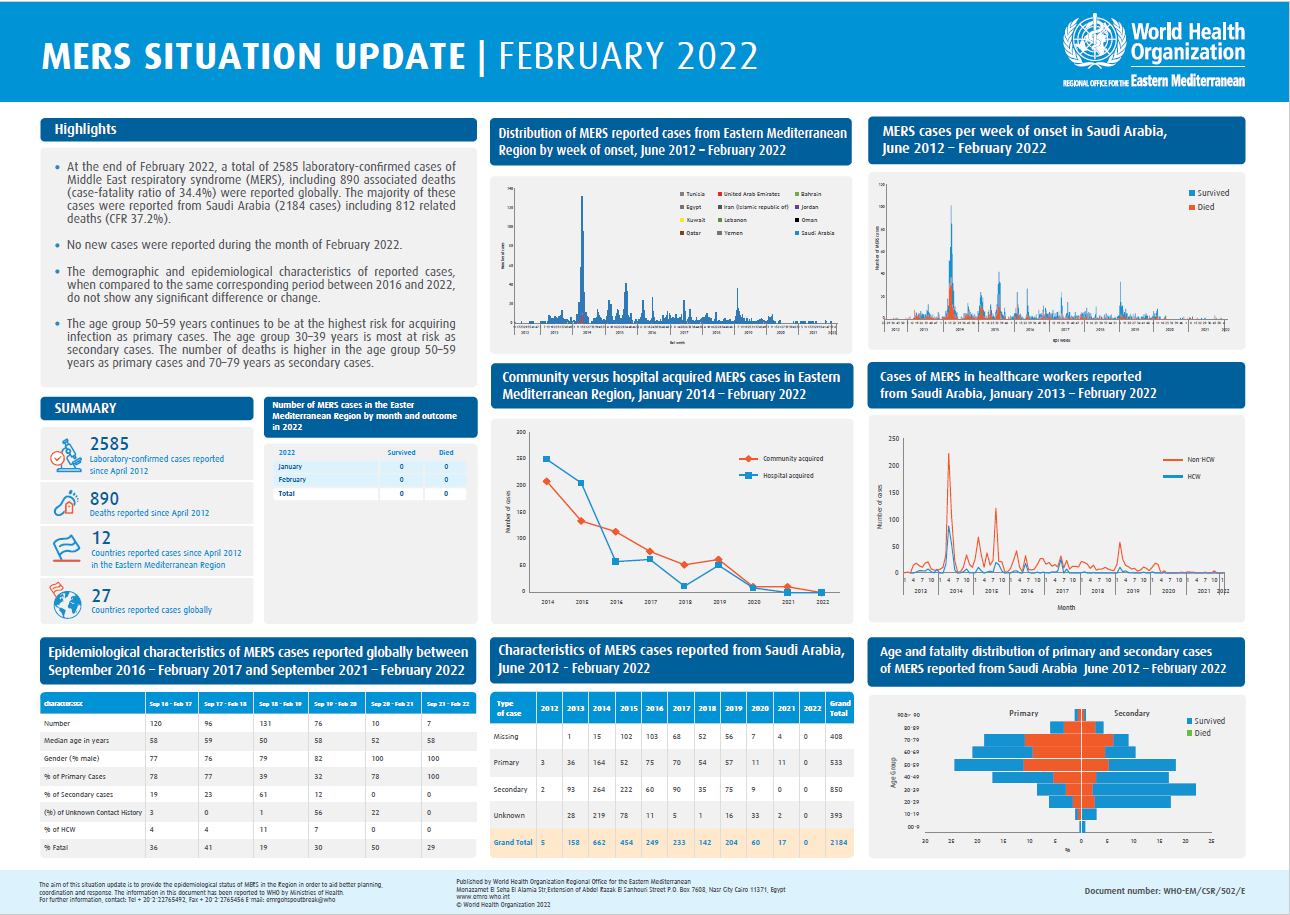
\includegraphics[width=15cm, height=15cm]{MERS.PNG}

\section{Epidemiologia do COVID-19}

O COVID-19 possui características muito semelhantes ao do SARS-CoV, fato que é observado no trabalho de Zhou e colaboradores (2020) ao comparar o COVID-19 com coronavirus de encontrados em morcegos foi possível encontrar uma relação de 96\% de proximidade entre eles. Por conta disso suspeita-se que teve origem em morcegos passando posteriormente a algum animal intermediário que após sofrer mutações foi possível a transmissão para humanos (Nogueira e Silva, 2020), embora haja essas suspeitas ainda não foi encontrado esse animal intermediário. 

A propagação do COVID-19 já era especulado que seria também por gotículas presentes na fala, em tosses e espirros, contato pessoal próximo, como toque, abraço ou aperto de mão; contato com objetos ou superfícies contaminadas, seguido de contato com a boca, nariz ou olhos características que os outros coronavirus possuem na sua transmissão. Entretanto sua propagação é muito superior aos outros da sua família. Além disso, segundo a Organização Mundial da Saúde (OMS) embora o período de incubação do SARS-CoV possa ser de 2-10 dias, o do COVID-19 pode variar entre 5-12 dias, pode ser um agravante adicional para a propagação do vírus, pois como foi observado Zhengdong e colaboradores (2020) e também por BAI e colaboradores (2020) já estava ocorrendo casos de possíveis pacientes assintomáticos transmitindo o vírus em fevereiro de 2020.

Dentre o grupos de pessoas mais propensas a terem complicações estão as pessoas com comorbidades e idosos (Galvão e Roncalli, 2020). Esses grupos estão em uma situação de vulnerabilidade maior e possuem uma maior probabilidade de desenvolver a forma mais grave da doença e até levar a óbito, sobretudo dentro desses grupos é classificado como mais vulnerável ainda os idosos acima de 80 anos.

O que tornou o vírus potencialmente destrutivo não foi sua mortalidade que em um contexto geral, segundo os dados da Organização Mundial da Saúde, ficou em torno de 1.2\%, mas também a sua alta disseminação gerando assim uma superlotação dos leitos por pacientes com a síndrome respiratória aguda grave que é o quadro mais grave da doença, além disso existem problemas cardíacos, neurológicos, hepáticos e intestinais associados a doença. Ao gerar o colapso do sistema de saúde, pacientes inclusive com outras doenças não poderiam ser atendidos como foi o caso da Itália primeiro bimestre de 2020.

Formas de prevenção para o COVID-19 e outras doenças virais são cuidados com a higiene como lavar as mãos e uso de máscara principalmente em locais com grande aglomerações. As máscaras são o primeiro cuidado que pode ser tomada para evitar o contágio, mas não somente isso, como apontado por SINCLAIR e colaboradores (2020) diminui a probabilidade que as próprias pessoas infectadas possuem transmitir o viros, muitos profissionais de saúde que tem contato frequente com pessoas potencialmente iniciam seus turnos e ao longo desse desenvolve sintomas leves e continua trabalhando.    

\section{COVID-19 como pandemia}

Diante da crescente propagação do vírus no dia 30 de janeiro de 2020, a Organização Mundial da Saúde(OMS) declarou que o surto do novo coronavírus constitui uma Emergência de Saúde Pública de Importância Internacional (ESPII), essa medida é caracterizada como avançada no controle ao vírus que se propagava por diversos países. Tal medida somente pode ser feito pelo diretor-geral da OMS, após realizar uma reunião com especialistas os quais o orientam sobre medidas emergências e para barrar o crescente número de casos do vírus. Esse estado de emergência de Saúde Pública busca a cooperação global para reduzir os casos da doença.

No dia 11 de março de 2020 o diretor-geral da OMS anunciou que o COVID-19, passaria a ser caracterizado como uma pandemia que é um termo que gera muitas incertezas e preocupações internacionais. Devido a sua propagação por mais de 114 países e que pandemia é caracterizada com relação a distribuição geográfica pelo mundo  no momento do seu anúncio os casos já ultrapassavam 118 mil casos.

\section{Modelo}

Um modelo é uma representação com um proposito de um sistema real no qual pode ser entendido como uma representação abstrata e mais simplificada de processos que ocorrem no mundo real, esses modelos buscam apresentar, analisar, compreender, explicar e até prever determinados fenômenos. O modelo é construído a partir da escolha dos parâmetros no qual o modelador analisa os dados e determina quais possuem um maior impacto na construção do modelo e quais dados são pouco relevantes para sua elaboração e construção, isso torna cada modelo essencialmente especial por ser construído por aspectos que o modelador acha relevante (Starfield ET AL. 1990) \cite{Qualitat24:online}. 

De outra forma pode ser entendido o modelo como uma representação de um sistema utilizando-se outro sistema com objetivo de facilitar o entendimento tanto por ser mais simples ou por possuir elementos mais conhecidos, além disso ambos apresentam funções semelhantes(Blackburn. 1997)\cite{blackburn}

\section{Modelagem de agentes e sistemas baseados em agentes}

A modelagem baseada em agentes (MBA) é uma metodologia usada para construir modelos formais de sistemas do mundo real que são compostos por unidades individuais que interagem repetidamente entre si e com seu ambiente.(Luis R. Izquierdo, Segismundo S. Izquierdo, William H. Sandholm. 2019)\cite{izquierdo2019introduction}. 

No entendimento de Bonabeau (2002) a MBA pode ser vista como conjunto de unidades autônomas que tomam suas decisões de forma individual baseadas em comportamentos, tais comportamentos são originados pela própria percepção sobre o ambiente e também sobre as interações geradas pelas outras unidades autônomas, essas unidades individuais podem ser chamadas de agentes. Estes podem ser capazes de evoluir, permitindo novos comportamentos e interações. Existe ainda a possibilidade da MBA utiliza-se de inteligencia artificial através de redes neurais, algoritmos evolucionários ou outras técnicas de aprendizado para permitir aprendizado e adaptação realistas\cite{bonabeau2002agent}. 

No mundo real assim como nas MBAs cada individuo desempenha um papel e suas interações individuais com outros e com o ambiente influenciarão o resultado que o grupo atingirá. A imagem abaixo mostra diversas interações entre pessoas e agentes computacionais.  


\figura{real_world}{Em um modelo baseado em agente, as unidades individuais do sistema do mundo real a ser modelado e suas interações são representadas de forma explícita e individual no modelo\cite{02Introd63:online}}{real_world}{width=0.75\textwidth}


As variáveis que moldam as interações entre os agentes assim como o comportamento desses agentes com o ambiente e com os demais indivíduos podem ser pensadas de forma mais simples ou elaboradas em contextos mais específicos ou complexos. Dessa forma pode-se observar também limitações na elaboração dos agentes e na construção modelo.

\section{Principais vantagens na Modelagem de agentes e Desafios}

A modelagem baseada em agentes(MBA) possibilita observar certos comportamentos individuais de humanos e animais que não seriam possíveis distinguir corretamente em sistemas complexos, essa capacidade de analisar comportamentos individuais transforma a observação sobre um fenômeno em uma visão mais simplificada, alguns dos exemplos para esses comportamentos podem ser observados em epidemias, movimento de animais em grupos coordenados, trânsito de veículos. Além disso destaca-se a alta flexibilidade desses Sistemas Baseados em Agentes, uma vez que é possível fazer alterações tanto no ambientes, quantos nos agentes que interagem entre si. Conforme Bonabeau(2002) mesmo modelos simples baseado em agentes pode exibir padrões de comportamento complexos e contribuir com informações valiosas sobre a dinâmica do sistema do mundo real que ele emula \cite{bonabeau2002agent}

\figura{Passaros}{Movimento dos pássaros coordenados em bando}{Passaros}{width=0.75\textwidth}

Axtell (2000) Afirma que a modelagem baseada em agentes pode ser a solução para alguns processos levando a uma compreensão melhor sobre o comportamento do modelo, além de possibilitar melhores testes, permitindo a elaboração de suposições com isso possibilitando novas hipóteses desconhecidas anteriormente.\cite{Axtell:online}

Um desafio, comum a todas as técnicas de modelagem, é que o modelo deve ser construído num nível correto de descrição dos fenômenos, usando uma quantidade adequada de detalhes, para servir ao seu propósito. Outro desafio envolve a utilização da MBA nas ciências sociais, que geralmente envolvem seres humanos com comportamentos potencialmente irracionais, de escolhas subjetivas e psicologia complexa, aspectos difíceis de quantificar, calibrar e muitas vezes justificar. Outro desafio está relacionado à própria definição da MBA, a qual trata um sistema no nível de suas unidades constituintes, o que exige elevado poder computacional e tempo para simulação do modelo, conforme a escala e a complexidade modelada.

\section{Geoprocessamento e Sistema de Informações Geográficas}

Geoprocessamento é a utilização de técnicas matemáticas e computacionais que tornam possível a realização de analises de informações geográficas, as quais são fundamentais em um pais igual ao Brasil. Além de ter um tamanho continental, carece de informações sobre as próprias características geográficas. Visando preservar a biodiversidade, conservar suas áreas prioritárias com potencialidades ecológicas, o Geoprocessamento é uma das tecnologias que tem sido utilizadas para preservar e proteger o território brasileiro.\cite{ximenes_modelagem_2008} \cite{georef:online}. 

As ferramentas que utilizam-se do Geoprocessamento são conhecidas como Sistemas de Informação Geográficas(SIG) ou Geographic Information System(GIS), podem ser entendidos como conjuntos de estruturas abrangendo programas computacionais, informações espaciais e hardwares possibilitando a analise e integração de diversos tipos de dados, criação de bancos, instituições, elaboração de mapas, documentos cartográficos\cite{Burrough:online}.

\figura{Geoprocessamento Imagem}{Componentes de um sistema de informação geográfica}{Geoprocessamento Imagem}{width=0.75\textwidth}



\section{Ferramenta de Sistema de Informações Geográficas }

Uma das ferramentas utilizadas na construção do trabalho foi o QGIS, seu nome tem origem em Quantum GIS (QGIS). Esse software faz parte do FOSS (Free and Open Source Software), logo uma das características marcantes do software é ser Código Aberto é gratuito\cite{Qgis:online} e pode ser baixado em diferentes sistemas operacionais como Linux, Mac, Windows. Além do mais conta com vários plugins desenvolvidos em varias linguagens sendo a principal Python. O software possui apoio da comunidade na construção e elaboração de projetos. Por fim dispõe de uma excelente integração com GAMA que foi a ferramenta principal utilizada na modelagem das simulações. 


